% Created by tikzDevice version 0.10.1 on 2018-06-30 09:32:04
% !TEX encoding = UTF-8 Unicode
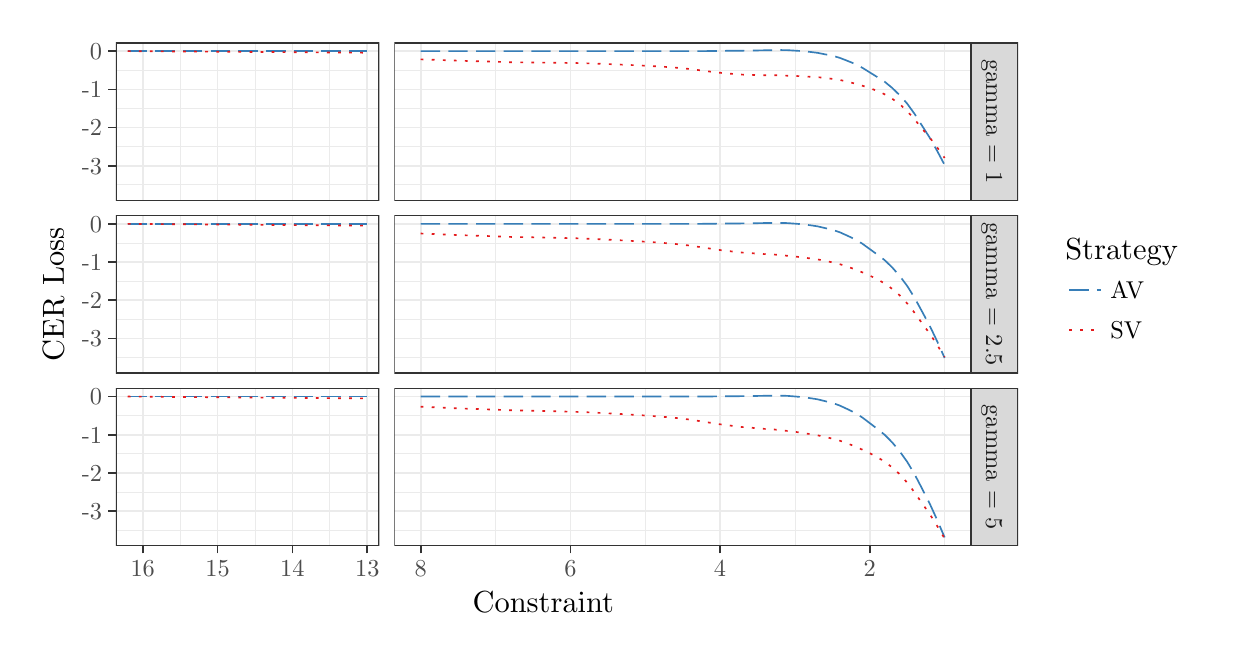
\begin{tikzpicture}[x=1pt,y=1pt]
\definecolor{fillColor}{RGB}{255,255,255}
\path[use as bounding box,fill=fillColor,fill opacity=0.00] (0,0) rectangle (426.79,216.81);
\begin{scope}
\path[clip] (  0.00,  0.00) rectangle (426.79,216.81);
\definecolor{drawColor}{RGB}{255,255,255}
\definecolor{fillColor}{RGB}{255,255,255}

\path[draw=drawColor,line width= 0.6pt,line join=round,line cap=round,fill=fillColor] (  0.00,  0.00) rectangle (426.79,216.81);
\end{scope}
\begin{scope}
\path[clip] ( 31.83,154.40) rectangle (127.04,211.31);
\definecolor{fillColor}{RGB}{255,255,255}

\path[fill=fillColor] ( 31.83,154.40) rectangle (127.04,211.31);
\definecolor{drawColor}{gray}{0.92}

\path[draw=drawColor,line width= 0.3pt,line join=round] ( 31.83,160.00) --
	(127.04,160.00);

\path[draw=drawColor,line width= 0.3pt,line join=round] ( 31.83,173.80) --
	(127.04,173.80);

\path[draw=drawColor,line width= 0.3pt,line join=round] ( 31.83,187.61) --
	(127.04,187.61);

\path[draw=drawColor,line width= 0.3pt,line join=round] ( 31.83,201.42) --
	(127.04,201.42);

\path[draw=drawColor,line width= 0.3pt,line join=round] (109.19,154.40) --
	(109.19,211.31);

\path[draw=drawColor,line width= 0.3pt,line join=round] ( 82.14,154.40) --
	( 82.14,211.31);

\path[draw=drawColor,line width= 0.3pt,line join=round] ( 55.09,154.40) --
	( 55.09,211.31);

\path[draw=drawColor,line width= 0.6pt,line join=round] ( 31.83,166.90) --
	(127.04,166.90);

\path[draw=drawColor,line width= 0.6pt,line join=round] ( 31.83,180.71) --
	(127.04,180.71);

\path[draw=drawColor,line width= 0.6pt,line join=round] ( 31.83,194.52) --
	(127.04,194.52);

\path[draw=drawColor,line width= 0.6pt,line join=round] ( 31.83,208.32) --
	(127.04,208.32);

\path[draw=drawColor,line width= 0.6pt,line join=round] (122.71,154.40) --
	(122.71,211.31);

\path[draw=drawColor,line width= 0.6pt,line join=round] ( 95.66,154.40) --
	( 95.66,211.31);

\path[draw=drawColor,line width= 0.6pt,line join=round] ( 68.61,154.40) --
	( 68.61,211.31);

\path[draw=drawColor,line width= 0.6pt,line join=round] ( 41.57,154.40) --
	( 41.57,211.31);
\definecolor{drawColor}{RGB}{55,126,184}

\path[draw=drawColor,line width= 0.6pt,dash pattern=on 7pt off 3pt ,line join=round] ( 36.16,208.32) --
	( 38.86,208.32) --
	( 41.57,208.32) --
	( 44.27,208.32) --
	( 46.98,208.32) --
	( 49.68,208.32) --
	( 52.39,208.32) --
	( 55.09,208.32) --
	( 57.80,208.32) --
	( 60.50,208.32) --
	( 63.21,208.32) --
	( 65.91,208.32) --
	( 68.61,208.32) --
	( 71.32,208.32) --
	( 74.02,208.32) --
	( 76.73,208.32) --
	( 79.43,208.32) --
	( 82.14,208.32) --
	( 84.84,208.32) --
	( 87.55,208.32) --
	( 90.25,208.32) --
	( 92.96,208.32) --
	( 95.66,208.32) --
	( 98.37,208.32) --
	(101.07,208.32) --
	(103.78,208.32) --
	(106.48,208.32) --
	(109.19,208.32) --
	(111.89,208.32) --
	(114.60,208.32) --
	(117.30,208.32) --
	(120.01,208.32) --
	(122.71,208.32);
\definecolor{drawColor}{RGB}{228,26,28}

\path[draw=drawColor,line width= 0.6pt,dash pattern=on 1pt off 3pt ,line join=round] ( 36.16,208.32) --
	( 38.86,208.31) --
	( 41.57,208.29) --
	( 44.27,208.27) --
	( 46.98,208.26) --
	( 49.68,208.24) --
	( 52.39,208.22) --
	( 55.09,208.21) --
	( 57.80,208.19) --
	( 60.50,208.17) --
	( 63.21,208.15) --
	( 65.91,208.14) --
	( 68.61,208.12) --
	( 71.32,208.10) --
	( 74.02,208.08) --
	( 76.73,208.07) --
	( 79.43,208.05) --
	( 82.14,208.03) --
	( 84.84,208.01) --
	( 87.55,208.00) --
	( 90.25,207.98) --
	( 92.96,207.96) --
	( 95.66,207.94) --
	( 98.37,207.92) --
	(101.07,207.91) --
	(103.78,207.89) --
	(106.48,207.87) --
	(109.19,207.85) --
	(111.89,207.83) --
	(114.60,207.82) --
	(117.30,207.80) --
	(120.01,207.78) --
	(122.71,207.76);
\definecolor{drawColor}{gray}{0.20}

\path[draw=drawColor,line width= 0.6pt,line join=round,line cap=round] ( 31.83,154.40) rectangle (127.04,211.31);
\end{scope}
\begin{scope}
\path[clip] ( 31.83, 91.99) rectangle (127.04,148.90);
\definecolor{fillColor}{RGB}{255,255,255}

\path[fill=fillColor] ( 31.83, 91.99) rectangle (127.04,148.90);
\definecolor{drawColor}{gray}{0.92}

\path[draw=drawColor,line width= 0.3pt,line join=round] ( 31.83, 97.59) --
	(127.04, 97.59);

\path[draw=drawColor,line width= 0.3pt,line join=round] ( 31.83,111.40) --
	(127.04,111.40);

\path[draw=drawColor,line width= 0.3pt,line join=round] ( 31.83,125.20) --
	(127.04,125.20);

\path[draw=drawColor,line width= 0.3pt,line join=round] ( 31.83,139.01) --
	(127.04,139.01);

\path[draw=drawColor,line width= 0.3pt,line join=round] (109.19, 91.99) --
	(109.19,148.90);

\path[draw=drawColor,line width= 0.3pt,line join=round] ( 82.14, 91.99) --
	( 82.14,148.90);

\path[draw=drawColor,line width= 0.3pt,line join=round] ( 55.09, 91.99) --
	( 55.09,148.90);

\path[draw=drawColor,line width= 0.6pt,line join=round] ( 31.83,104.49) --
	(127.04,104.49);

\path[draw=drawColor,line width= 0.6pt,line join=round] ( 31.83,118.30) --
	(127.04,118.30);

\path[draw=drawColor,line width= 0.6pt,line join=round] ( 31.83,132.11) --
	(127.04,132.11);

\path[draw=drawColor,line width= 0.6pt,line join=round] ( 31.83,145.92) --
	(127.04,145.92);

\path[draw=drawColor,line width= 0.6pt,line join=round] (122.71, 91.99) --
	(122.71,148.90);

\path[draw=drawColor,line width= 0.6pt,line join=round] ( 95.66, 91.99) --
	( 95.66,148.90);

\path[draw=drawColor,line width= 0.6pt,line join=round] ( 68.61, 91.99) --
	( 68.61,148.90);

\path[draw=drawColor,line width= 0.6pt,line join=round] ( 41.57, 91.99) --
	( 41.57,148.90);
\definecolor{drawColor}{RGB}{55,126,184}

\path[draw=drawColor,line width= 0.6pt,dash pattern=on 7pt off 3pt ,line join=round] ( 36.16,145.92) --
	( 38.86,145.92) --
	( 41.57,145.92) --
	( 44.27,145.92) --
	( 46.98,145.92) --
	( 49.68,145.92) --
	( 52.39,145.92) --
	( 55.09,145.92) --
	( 57.80,145.92) --
	( 60.50,145.92) --
	( 63.21,145.92) --
	( 65.91,145.92) --
	( 68.61,145.92) --
	( 71.32,145.92) --
	( 74.02,145.92) --
	( 76.73,145.92) --
	( 79.43,145.92) --
	( 82.14,145.92) --
	( 84.84,145.92) --
	( 87.55,145.92) --
	( 90.25,145.92) --
	( 92.96,145.92) --
	( 95.66,145.92) --
	( 98.37,145.92) --
	(101.07,145.92) --
	(103.78,145.92) --
	(106.48,145.92) --
	(109.19,145.92) --
	(111.89,145.92) --
	(114.60,145.92) --
	(117.30,145.92) --
	(120.01,145.92) --
	(122.71,145.92);
\definecolor{drawColor}{RGB}{228,26,28}

\path[draw=drawColor,line width= 0.6pt,dash pattern=on 1pt off 3pt ,line join=round] ( 36.16,145.92) --
	( 38.86,145.90) --
	( 41.57,145.88) --
	( 44.27,145.86) --
	( 46.98,145.84) --
	( 49.68,145.82) --
	( 52.39,145.80) --
	( 55.09,145.78) --
	( 57.80,145.76) --
	( 60.50,145.74) --
	( 63.21,145.72) --
	( 65.91,145.70) --
	( 68.61,145.68) --
	( 71.32,145.66) --
	( 74.02,145.64) --
	( 76.73,145.62) --
	( 79.43,145.59) --
	( 82.14,145.57) --
	( 84.84,145.55) --
	( 87.55,145.53) --
	( 90.25,145.51) --
	( 92.96,145.49) --
	( 95.66,145.47) --
	( 98.37,145.45) --
	(101.07,145.43) --
	(103.78,145.41) --
	(106.48,145.39) --
	(109.19,145.37) --
	(111.89,145.35) --
	(114.60,145.33) --
	(117.30,145.31) --
	(120.01,145.29) --
	(122.71,145.27);
\definecolor{drawColor}{gray}{0.20}

\path[draw=drawColor,line width= 0.6pt,line join=round,line cap=round] ( 31.83, 91.99) rectangle (127.04,148.90);
\end{scope}
\begin{scope}
\path[clip] ( 31.83, 29.59) rectangle (127.04, 86.49);
\definecolor{fillColor}{RGB}{255,255,255}

\path[fill=fillColor] ( 31.83, 29.59) rectangle (127.04, 86.49);
\definecolor{drawColor}{gray}{0.92}

\path[draw=drawColor,line width= 0.3pt,line join=round] ( 31.83, 35.18) --
	(127.04, 35.18);

\path[draw=drawColor,line width= 0.3pt,line join=round] ( 31.83, 48.99) --
	(127.04, 48.99);

\path[draw=drawColor,line width= 0.3pt,line join=round] ( 31.83, 62.80) --
	(127.04, 62.80);

\path[draw=drawColor,line width= 0.3pt,line join=round] ( 31.83, 76.60) --
	(127.04, 76.60);

\path[draw=drawColor,line width= 0.3pt,line join=round] (109.19, 29.59) --
	(109.19, 86.49);

\path[draw=drawColor,line width= 0.3pt,line join=round] ( 82.14, 29.59) --
	( 82.14, 86.49);

\path[draw=drawColor,line width= 0.3pt,line join=round] ( 55.09, 29.59) --
	( 55.09, 86.49);

\path[draw=drawColor,line width= 0.6pt,line join=round] ( 31.83, 42.08) --
	(127.04, 42.08);

\path[draw=drawColor,line width= 0.6pt,line join=round] ( 31.83, 55.89) --
	(127.04, 55.89);

\path[draw=drawColor,line width= 0.6pt,line join=round] ( 31.83, 69.70) --
	(127.04, 69.70);

\path[draw=drawColor,line width= 0.6pt,line join=round] ( 31.83, 83.51) --
	(127.04, 83.51);

\path[draw=drawColor,line width= 0.6pt,line join=round] (122.71, 29.59) --
	(122.71, 86.49);

\path[draw=drawColor,line width= 0.6pt,line join=round] ( 95.66, 29.59) --
	( 95.66, 86.49);

\path[draw=drawColor,line width= 0.6pt,line join=round] ( 68.61, 29.59) --
	( 68.61, 86.49);

\path[draw=drawColor,line width= 0.6pt,line join=round] ( 41.57, 29.59) --
	( 41.57, 86.49);
\definecolor{drawColor}{RGB}{55,126,184}

\path[draw=drawColor,line width= 0.6pt,dash pattern=on 7pt off 3pt ,line join=round] ( 36.16, 83.51) --
	( 36.16, 83.51) --
	( 36.16, 83.51) --
	( 38.86, 83.51) --
	( 38.86, 83.51) --
	( 38.86, 83.51) --
	( 41.57, 83.51) --
	( 41.57, 83.51) --
	( 41.57, 83.51) --
	( 44.27, 83.51) --
	( 44.27, 83.51) --
	( 44.27, 83.51) --
	( 46.98, 83.51) --
	( 46.98, 83.51) --
	( 46.98, 83.51) --
	( 49.68, 83.51) --
	( 49.68, 83.51) --
	( 49.68, 83.51) --
	( 52.39, 83.51) --
	( 52.39, 83.51) --
	( 52.39, 83.51) --
	( 55.09, 83.51) --
	( 55.09, 83.51) --
	( 55.09, 83.51) --
	( 57.80, 83.51) --
	( 57.80, 83.51) --
	( 57.80, 83.51) --
	( 60.50, 83.51) --
	( 60.50, 83.51) --
	( 60.50, 83.51) --
	( 63.21, 83.51) --
	( 63.21, 83.51) --
	( 63.21, 83.51) --
	( 65.91, 83.51) --
	( 65.91, 83.51) --
	( 65.91, 83.51) --
	( 68.61, 83.51) --
	( 68.61, 83.51) --
	( 68.61, 83.51) --
	( 71.32, 83.51) --
	( 71.32, 83.51) --
	( 71.32, 83.51) --
	( 74.02, 83.51) --
	( 74.02, 83.51) --
	( 74.02, 83.51) --
	( 76.73, 83.51) --
	( 76.73, 83.51) --
	( 76.73, 83.51) --
	( 79.43, 83.51) --
	( 79.43, 83.51) --
	( 79.43, 83.51) --
	( 82.14, 83.51) --
	( 82.14, 83.51) --
	( 82.14, 83.51) --
	( 84.84, 83.51) --
	( 84.84, 83.51) --
	( 84.84, 83.51) --
	( 87.55, 83.51) --
	( 87.55, 83.51) --
	( 87.55, 83.51) --
	( 90.25, 83.51) --
	( 90.25, 83.51) --
	( 90.25, 83.51) --
	( 92.96, 83.51) --
	( 92.96, 83.51) --
	( 92.96, 83.51) --
	( 95.66, 83.51) --
	( 95.66, 83.51) --
	( 95.66, 83.51) --
	( 98.37, 83.51) --
	( 98.37, 83.51) --
	( 98.37, 83.51) --
	(101.07, 83.51) --
	(101.07, 83.51) --
	(101.07, 83.51) --
	(103.78, 83.51) --
	(103.78, 83.51) --
	(103.78, 83.51) --
	(106.48, 83.51) --
	(106.48, 83.51) --
	(106.48, 83.51) --
	(109.19, 83.51) --
	(109.19, 83.51) --
	(109.19, 83.51) --
	(111.89, 83.51) --
	(111.89, 83.51) --
	(111.89, 83.51) --
	(114.60, 83.51) --
	(114.60, 83.51) --
	(114.60, 83.51) --
	(117.30, 83.51) --
	(117.30, 83.51) --
	(117.30, 83.51) --
	(120.01, 83.51) --
	(120.01, 83.51) --
	(120.01, 83.51) --
	(122.71, 83.51) --
	(122.71, 83.51) --
	(122.71, 83.51);
\definecolor{drawColor}{RGB}{228,26,28}

\path[draw=drawColor,line width= 0.6pt,dash pattern=on 1pt off 3pt ,line join=round] ( 36.16, 83.51) --
	( 38.86, 83.49) --
	( 41.57, 83.47) --
	( 44.27, 83.45) --
	( 46.98, 83.43) --
	( 49.68, 83.40) --
	( 52.39, 83.38) --
	( 55.09, 83.36) --
	( 57.80, 83.34) --
	( 60.50, 83.32) --
	( 63.21, 83.30) --
	( 65.91, 83.28) --
	( 68.61, 83.26) --
	( 71.32, 83.24) --
	( 74.02, 83.21) --
	( 76.73, 83.19) --
	( 79.43, 83.17) --
	( 82.14, 83.15) --
	( 84.84, 83.13) --
	( 87.55, 83.11) --
	( 90.25, 83.09) --
	( 92.96, 83.07) --
	( 95.66, 83.04) --
	( 98.37, 83.02) --
	(101.07, 83.00) --
	(103.78, 82.98) --
	(106.48, 82.96) --
	(109.19, 82.94) --
	(111.89, 82.92) --
	(114.60, 82.90) --
	(117.30, 82.87) --
	(120.01, 82.85) --
	(122.71, 82.83);
\definecolor{drawColor}{gray}{0.20}

\path[draw=drawColor,line width= 0.6pt,line join=round,line cap=round] ( 31.83, 29.59) rectangle (127.04, 86.49);
\end{scope}
\begin{scope}
\path[clip] (132.54,154.40) rectangle (340.81,211.31);
\definecolor{fillColor}{RGB}{255,255,255}

\path[fill=fillColor] (132.54,154.40) rectangle (340.81,211.31);
\definecolor{drawColor}{gray}{0.92}

\path[draw=drawColor,line width= 0.3pt,line join=round] (132.54,160.00) --
	(340.81,160.00);

\path[draw=drawColor,line width= 0.3pt,line join=round] (132.54,173.80) --
	(340.81,173.80);

\path[draw=drawColor,line width= 0.3pt,line join=round] (132.54,187.61) --
	(340.81,187.61);

\path[draw=drawColor,line width= 0.3pt,line join=round] (132.54,201.42) --
	(340.81,201.42);

\path[draw=drawColor,line width= 0.3pt,line join=round] (331.34,154.40) --
	(331.34,211.31);

\path[draw=drawColor,line width= 0.3pt,line join=round] (277.25,154.40) --
	(277.25,211.31);

\path[draw=drawColor,line width= 0.3pt,line join=round] (223.15,154.40) --
	(223.15,211.31);

\path[draw=drawColor,line width= 0.3pt,line join=round] (169.05,154.40) --
	(169.05,211.31);

\path[draw=drawColor,line width= 0.6pt,line join=round] (132.54,166.90) --
	(340.81,166.90);

\path[draw=drawColor,line width= 0.6pt,line join=round] (132.54,180.71) --
	(340.81,180.71);

\path[draw=drawColor,line width= 0.6pt,line join=round] (132.54,194.52) --
	(340.81,194.52);

\path[draw=drawColor,line width= 0.6pt,line join=round] (132.54,208.32) --
	(340.81,208.32);

\path[draw=drawColor,line width= 0.6pt,line join=round] (304.29,154.40) --
	(304.29,211.31);

\path[draw=drawColor,line width= 0.6pt,line join=round] (250.20,154.40) --
	(250.20,211.31);

\path[draw=drawColor,line width= 0.6pt,line join=round] (196.10,154.40) --
	(196.10,211.31);

\path[draw=drawColor,line width= 0.6pt,line join=round] (142.01,154.40) --
	(142.01,211.31);
\definecolor{drawColor}{RGB}{55,126,184}

\path[draw=drawColor,line width= 0.6pt,dash pattern=on 7pt off 3pt ,line join=round] (142.01,208.32) --
	(144.71,208.32) --
	(147.42,208.32) --
	(150.12,208.32) --
	(152.82,208.32) --
	(155.53,208.32) --
	(158.23,208.32) --
	(160.94,208.32) --
	(163.64,208.32) --
	(166.35,208.32) --
	(169.05,208.32) --
	(171.76,208.32) --
	(174.46,208.32) --
	(177.17,208.32) --
	(179.87,208.32) --
	(182.58,208.32) --
	(185.28,208.32) --
	(187.99,208.32) --
	(190.69,208.32) --
	(193.40,208.32) --
	(196.10,208.32) --
	(198.81,208.32) --
	(201.51,208.32) --
	(204.22,208.32) --
	(206.92,208.32) --
	(209.63,208.32) --
	(212.33,208.32) --
	(215.04,208.32) --
	(217.74,208.32) --
	(220.44,208.32) --
	(223.15,208.32) --
	(225.85,208.32) --
	(228.56,208.32) --
	(231.26,208.32) --
	(233.97,208.32) --
	(236.67,208.32) --
	(239.38,208.32) --
	(242.08,208.32) --
	(244.79,208.34) --
	(247.49,208.38) --
	(250.20,208.41) --
	(252.90,208.45) --
	(255.61,208.47) --
	(258.31,208.49) --
	(261.02,208.54) --
	(263.72,208.58) --
	(266.43,208.63) --
	(269.13,208.68) --
	(271.84,208.72) --
	(274.54,208.68) --
	(277.25,208.51) --
	(279.95,208.33) --
	(282.66,208.06) --
	(285.36,207.72) --
	(288.06,207.19) --
	(290.77,206.69) --
	(293.47,205.89) --
	(296.18,204.84) --
	(298.88,203.75) --
	(301.59,202.33) --
	(304.29,200.64) --
	(307.00,198.96) --
	(309.70,197.25) --
	(312.41,195.02) --
	(315.11,192.39) --
	(317.82,189.34) --
	(320.52,185.60) --
	(323.23,181.31) --
	(325.93,177.09) --
	(328.64,172.28) --
	(331.34,167.19);
\definecolor{drawColor}{RGB}{228,26,28}

\path[draw=drawColor,line width= 0.6pt,dash pattern=on 1pt off 3pt ,line join=round] (142.01,205.36) --
	(144.71,205.27) --
	(147.42,205.18) --
	(150.12,205.08) --
	(152.82,204.98) --
	(155.53,204.89) --
	(158.23,204.80) --
	(160.94,204.72) --
	(163.64,204.65) --
	(166.35,204.57) --
	(169.05,204.50) --
	(171.76,204.41) --
	(174.46,204.32) --
	(177.17,204.28) --
	(179.87,204.27) --
	(182.58,204.24) --
	(185.28,204.20) --
	(187.99,204.17) --
	(190.69,204.13) --
	(193.40,204.09) --
	(196.10,204.05) --
	(198.81,204.01) --
	(201.51,203.94) --
	(204.22,203.85) --
	(206.92,203.76) --
	(209.63,203.66) --
	(212.33,203.55) --
	(215.04,203.43) --
	(217.74,203.31) --
	(220.44,203.20) --
	(223.15,203.05) --
	(225.85,202.91) --
	(228.56,202.76) --
	(231.26,202.58) --
	(233.97,202.38) --
	(236.67,202.13) --
	(239.38,201.86) --
	(242.08,201.52) --
	(244.79,201.17) --
	(247.49,200.82) --
	(250.20,200.51) --
	(252.90,200.27) --
	(255.61,200.03) --
	(258.31,199.83) --
	(261.02,199.79) --
	(263.72,199.64) --
	(266.43,199.63) --
	(269.13,199.66) --
	(271.84,199.57) --
	(274.54,199.45) --
	(277.25,199.36) --
	(279.95,199.23) --
	(282.66,199.08) --
	(285.36,198.91) --
	(288.06,198.70) --
	(290.77,198.29) --
	(293.47,197.91) --
	(296.18,197.31) --
	(298.88,196.63) --
	(301.59,195.83) --
	(304.29,194.94) --
	(307.00,193.97) --
	(309.70,192.70) --
	(312.41,191.11) --
	(315.11,189.18) --
	(317.82,186.65) --
	(320.52,183.65) --
	(323.23,180.27) --
	(325.93,177.14) --
	(328.64,173.54) --
	(331.34,169.73);
\definecolor{drawColor}{gray}{0.20}

\path[draw=drawColor,line width= 0.6pt,line join=round,line cap=round] (132.54,154.40) rectangle (340.81,211.31);
\end{scope}
\begin{scope}
\path[clip] (132.54, 91.99) rectangle (340.81,148.90);
\definecolor{fillColor}{RGB}{255,255,255}

\path[fill=fillColor] (132.54, 91.99) rectangle (340.81,148.90);
\definecolor{drawColor}{gray}{0.92}

\path[draw=drawColor,line width= 0.3pt,line join=round] (132.54, 97.59) --
	(340.81, 97.59);

\path[draw=drawColor,line width= 0.3pt,line join=round] (132.54,111.40) --
	(340.81,111.40);

\path[draw=drawColor,line width= 0.3pt,line join=round] (132.54,125.20) --
	(340.81,125.20);

\path[draw=drawColor,line width= 0.3pt,line join=round] (132.54,139.01) --
	(340.81,139.01);

\path[draw=drawColor,line width= 0.3pt,line join=round] (331.34, 91.99) --
	(331.34,148.90);

\path[draw=drawColor,line width= 0.3pt,line join=round] (277.25, 91.99) --
	(277.25,148.90);

\path[draw=drawColor,line width= 0.3pt,line join=round] (223.15, 91.99) --
	(223.15,148.90);

\path[draw=drawColor,line width= 0.3pt,line join=round] (169.05, 91.99) --
	(169.05,148.90);

\path[draw=drawColor,line width= 0.6pt,line join=round] (132.54,104.49) --
	(340.81,104.49);

\path[draw=drawColor,line width= 0.6pt,line join=round] (132.54,118.30) --
	(340.81,118.30);

\path[draw=drawColor,line width= 0.6pt,line join=round] (132.54,132.11) --
	(340.81,132.11);

\path[draw=drawColor,line width= 0.6pt,line join=round] (132.54,145.92) --
	(340.81,145.92);

\path[draw=drawColor,line width= 0.6pt,line join=round] (304.29, 91.99) --
	(304.29,148.90);

\path[draw=drawColor,line width= 0.6pt,line join=round] (250.20, 91.99) --
	(250.20,148.90);

\path[draw=drawColor,line width= 0.6pt,line join=round] (196.10, 91.99) --
	(196.10,148.90);

\path[draw=drawColor,line width= 0.6pt,line join=round] (142.01, 91.99) --
	(142.01,148.90);
\definecolor{drawColor}{RGB}{55,126,184}

\path[draw=drawColor,line width= 0.6pt,dash pattern=on 7pt off 3pt ,line join=round] (142.01,145.92) --
	(144.71,145.92) --
	(147.42,145.92) --
	(150.12,145.92) --
	(152.82,145.92) --
	(155.53,145.92) --
	(158.23,145.92) --
	(160.94,145.92) --
	(163.64,145.92) --
	(166.35,145.92) --
	(169.05,145.92) --
	(171.76,145.92) --
	(174.46,145.92) --
	(177.17,145.92) --
	(179.87,145.92) --
	(182.58,145.92) --
	(185.28,145.92) --
	(187.99,145.92) --
	(190.69,145.92) --
	(193.40,145.92) --
	(196.10,145.92) --
	(198.81,145.92) --
	(201.51,145.92) --
	(204.22,145.92) --
	(206.92,145.92) --
	(209.63,145.92) --
	(212.33,145.92) --
	(215.04,145.92) --
	(217.74,145.92) --
	(220.44,145.92) --
	(223.15,145.92) --
	(225.85,145.92) --
	(228.56,145.92) --
	(231.26,145.92) --
	(233.97,145.92) --
	(236.67,145.92) --
	(239.38,145.92) --
	(242.08,145.92) --
	(244.79,145.93) --
	(247.49,145.97) --
	(250.20,146.00) --
	(252.90,146.03) --
	(255.61,146.06) --
	(258.31,146.08) --
	(261.02,146.12) --
	(263.72,146.16) --
	(266.43,146.21) --
	(269.13,146.25) --
	(271.84,146.26) --
	(274.54,146.19) --
	(277.25,145.99) --
	(279.95,145.76) --
	(282.66,145.43) --
	(285.36,145.03) --
	(288.06,144.41) --
	(290.77,143.80) --
	(293.47,142.87) --
	(296.18,141.65) --
	(298.88,140.38) --
	(301.59,138.76) --
	(304.29,136.80) --
	(307.00,134.82) --
	(309.70,132.78) --
	(312.41,130.16) --
	(315.11,127.08) --
	(317.82,123.48) --
	(320.52,119.13) --
	(323.23,114.15) --
	(325.93,109.13) --
	(328.64,103.47) --
	(331.34, 97.46);
\definecolor{drawColor}{RGB}{228,26,28}

\path[draw=drawColor,line width= 0.6pt,dash pattern=on 1pt off 3pt ,line join=round] (142.01,142.42) --
	(144.71,142.32) --
	(147.42,142.21) --
	(150.12,142.10) --
	(152.82,141.98) --
	(155.53,141.87) --
	(158.23,141.77) --
	(160.94,141.67) --
	(163.64,141.59) --
	(166.35,141.50) --
	(169.05,141.41) --
	(171.76,141.30) --
	(174.46,141.20) --
	(177.17,141.14) --
	(179.87,141.10) --
	(182.58,141.05) --
	(185.28,140.99) --
	(187.99,140.93) --
	(190.69,140.87) --
	(193.40,140.81) --
	(196.10,140.74) --
	(198.81,140.68) --
	(201.51,140.58) --
	(204.22,140.46) --
	(206.92,140.35) --
	(209.63,140.21) --
	(212.33,140.07) --
	(215.04,139.93) --
	(217.74,139.78) --
	(220.44,139.64) --
	(223.15,139.46) --
	(225.85,139.28) --
	(228.56,139.10) --
	(231.26,138.89) --
	(233.97,138.65) --
	(236.67,138.37) --
	(239.38,138.05) --
	(242.08,137.66) --
	(244.79,137.25) --
	(247.49,136.84) --
	(250.20,136.45) --
	(252.90,136.13) --
	(255.61,135.81) --
	(258.31,135.53) --
	(261.02,135.38) --
	(263.72,135.12) --
	(266.43,134.98) --
	(269.13,134.87) --
	(271.84,134.66) --
	(274.54,134.37) --
	(277.25,134.12) --
	(279.95,133.79) --
	(282.66,133.44) --
	(285.36,133.06) --
	(288.06,132.63) --
	(290.77,131.99) --
	(293.47,131.35) --
	(296.18,130.47) --
	(298.88,129.50) --
	(301.59,128.40) --
	(304.29,127.21) --
	(307.00,125.92) --
	(309.70,124.33) --
	(312.41,122.40) --
	(315.11,120.08) --
	(317.82,117.15) --
	(320.52,113.73) --
	(323.23,109.93) --
	(325.93,106.31) --
	(328.64,102.17) --
	(331.34, 97.77);
\definecolor{drawColor}{gray}{0.20}

\path[draw=drawColor,line width= 0.6pt,line join=round,line cap=round] (132.54, 91.99) rectangle (340.81,148.90);
\end{scope}
\begin{scope}
\path[clip] (132.54, 29.59) rectangle (340.81, 86.49);
\definecolor{fillColor}{RGB}{255,255,255}

\path[fill=fillColor] (132.54, 29.59) rectangle (340.81, 86.49);
\definecolor{drawColor}{gray}{0.92}

\path[draw=drawColor,line width= 0.3pt,line join=round] (132.54, 35.18) --
	(340.81, 35.18);

\path[draw=drawColor,line width= 0.3pt,line join=round] (132.54, 48.99) --
	(340.81, 48.99);

\path[draw=drawColor,line width= 0.3pt,line join=round] (132.54, 62.80) --
	(340.81, 62.80);

\path[draw=drawColor,line width= 0.3pt,line join=round] (132.54, 76.60) --
	(340.81, 76.60);

\path[draw=drawColor,line width= 0.3pt,line join=round] (331.34, 29.59) --
	(331.34, 86.49);

\path[draw=drawColor,line width= 0.3pt,line join=round] (277.25, 29.59) --
	(277.25, 86.49);

\path[draw=drawColor,line width= 0.3pt,line join=round] (223.15, 29.59) --
	(223.15, 86.49);

\path[draw=drawColor,line width= 0.3pt,line join=round] (169.05, 29.59) --
	(169.05, 86.49);

\path[draw=drawColor,line width= 0.6pt,line join=round] (132.54, 42.08) --
	(340.81, 42.08);

\path[draw=drawColor,line width= 0.6pt,line join=round] (132.54, 55.89) --
	(340.81, 55.89);

\path[draw=drawColor,line width= 0.6pt,line join=round] (132.54, 69.70) --
	(340.81, 69.70);

\path[draw=drawColor,line width= 0.6pt,line join=round] (132.54, 83.51) --
	(340.81, 83.51);

\path[draw=drawColor,line width= 0.6pt,line join=round] (304.29, 29.59) --
	(304.29, 86.49);

\path[draw=drawColor,line width= 0.6pt,line join=round] (250.20, 29.59) --
	(250.20, 86.49);

\path[draw=drawColor,line width= 0.6pt,line join=round] (196.10, 29.59) --
	(196.10, 86.49);

\path[draw=drawColor,line width= 0.6pt,line join=round] (142.01, 29.59) --
	(142.01, 86.49);
\definecolor{drawColor}{RGB}{55,126,184}

\path[draw=drawColor,line width= 0.6pt,dash pattern=on 7pt off 3pt ,line join=round] (142.01, 83.51) --
	(142.01, 83.51) --
	(142.01, 83.51) --
	(144.71, 83.51) --
	(144.71, 83.51) --
	(144.71, 83.51) --
	(147.42, 83.51) --
	(147.42, 83.51) --
	(147.42, 83.51) --
	(150.12, 83.51) --
	(150.12, 83.51) --
	(150.12, 83.51) --
	(152.82, 83.51) --
	(152.82, 83.51) --
	(152.82, 83.51) --
	(155.53, 83.51) --
	(155.53, 83.51) --
	(155.53, 83.51) --
	(158.23, 83.51) --
	(158.23, 83.51) --
	(158.23, 83.51) --
	(160.94, 83.51) --
	(160.94, 83.51) --
	(160.94, 83.51) --
	(163.64, 83.51) --
	(163.64, 83.51) --
	(163.64, 83.51) --
	(166.35, 83.51) --
	(166.35, 83.51) --
	(166.35, 83.51) --
	(169.05, 83.51) --
	(169.05, 83.51) --
	(169.05, 83.51) --
	(171.76, 83.51) --
	(171.76, 83.51) --
	(171.76, 83.51) --
	(174.46, 83.51) --
	(174.46, 83.51) --
	(174.46, 83.51) --
	(177.17, 83.51) --
	(177.17, 83.51) --
	(177.17, 83.51) --
	(179.87, 83.51) --
	(179.87, 83.51) --
	(179.87, 83.51) --
	(182.58, 83.51) --
	(182.58, 83.51) --
	(182.58, 83.51) --
	(185.28, 83.51) --
	(185.28, 83.51) --
	(185.28, 83.51) --
	(187.99, 83.51) --
	(187.99, 83.51) --
	(187.99, 83.51) --
	(190.69, 83.51) --
	(190.69, 83.51) --
	(190.69, 83.51) --
	(193.40, 83.51) --
	(193.40, 83.51) --
	(193.40, 83.51) --
	(196.10, 83.51) --
	(196.10, 83.51) --
	(196.10, 83.51) --
	(198.81, 83.51) --
	(198.81, 83.51) --
	(198.81, 83.51) --
	(201.51, 83.51) --
	(201.51, 83.51) --
	(201.51, 83.51) --
	(204.22, 83.51) --
	(204.22, 83.51) --
	(204.22, 83.51) --
	(206.92, 83.51) --
	(206.92, 83.51) --
	(206.92, 83.51) --
	(209.63, 83.51) --
	(209.63, 83.51) --
	(209.63, 83.51) --
	(212.33, 83.51) --
	(212.33, 83.51) --
	(212.33, 83.51) --
	(215.04, 83.51) --
	(215.04, 83.51) --
	(215.04, 83.51) --
	(217.74, 83.51) --
	(217.74, 83.51) --
	(217.74, 83.51) --
	(220.44, 83.51) --
	(220.44, 83.51) --
	(220.44, 83.51) --
	(223.15, 83.51) --
	(223.15, 83.51) --
	(223.15, 83.51) --
	(225.85, 83.51) --
	(225.85, 83.51) --
	(225.85, 83.51) --
	(228.56, 83.51) --
	(228.56, 83.51) --
	(228.56, 83.51) --
	(231.26, 83.51) --
	(231.26, 83.51) --
	(231.26, 83.51) --
	(233.97, 83.51) --
	(233.97, 83.51) --
	(233.97, 83.51) --
	(236.67, 83.51) --
	(236.67, 83.51) --
	(236.67, 83.51) --
	(239.38, 83.51) --
	(239.38, 83.51) --
	(239.38, 83.51) --
	(242.08, 83.51) --
	(242.08, 83.51) --
	(242.08, 83.51) --
	(244.79, 83.53) --
	(244.79, 83.53) --
	(244.79, 83.53) --
	(247.49, 83.56) --
	(247.49, 83.56) --
	(247.49, 83.56) --
	(250.20, 83.59) --
	(250.20, 83.59) --
	(250.20, 83.59) --
	(252.90, 83.62) --
	(252.90, 83.62) --
	(252.90, 83.62) --
	(255.61, 83.64) --
	(255.61, 83.64) --
	(255.61, 83.64) --
	(258.31, 83.66) --
	(258.31, 83.66) --
	(258.31, 83.66) --
	(261.02, 83.70) --
	(261.02, 83.70) --
	(261.02, 83.70) --
	(263.72, 83.74) --
	(263.72, 83.74) --
	(263.72, 83.74) --
	(266.43, 83.79) --
	(266.43, 83.79) --
	(266.43, 83.79) --
	(269.13, 83.83) --
	(269.13, 83.83) --
	(269.13, 83.83) --
	(271.84, 83.84) --
	(271.84, 83.84) --
	(271.84, 83.84) --
	(274.54, 83.76) --
	(274.54, 83.76) --
	(274.54, 83.76) --
	(277.25, 83.55) --
	(277.25, 83.55) --
	(277.25, 83.55) --
	(279.95, 83.29) --
	(279.95, 83.29) --
	(279.95, 83.29) --
	(282.66, 82.95) --
	(282.66, 82.95) --
	(282.66, 82.95) --
	(285.36, 82.53) --
	(285.36, 82.53) --
	(285.36, 82.53) --
	(288.06, 81.87) --
	(288.06, 81.87) --
	(288.06, 81.87) --
	(290.77, 81.23) --
	(290.77, 81.23) --
	(290.77, 81.23) --
	(293.47, 80.25) --
	(293.47, 80.25) --
	(293.47, 80.25) --
	(296.18, 78.99) --
	(296.18, 78.99) --
	(296.18, 78.99) --
	(298.88, 77.65) --
	(298.88, 77.65) --
	(298.88, 77.65) --
	(301.59, 75.96) --
	(301.59, 75.96) --
	(301.59, 75.96) --
	(304.29, 73.91) --
	(304.29, 73.91) --
	(304.29, 73.91) --
	(307.00, 71.84) --
	(307.00, 71.84) --
	(307.00, 71.84) --
	(309.70, 69.68) --
	(309.70, 69.68) --
	(309.70, 69.68) --
	(312.41, 66.93) --
	(312.41, 66.93) --
	(312.41, 66.93) --
	(315.11, 63.70) --
	(315.11, 63.70) --
	(315.11, 63.70) --
	(317.82, 59.92) --
	(317.82, 59.92) --
	(317.82, 59.92) --
	(320.52, 55.37) --
	(320.52, 55.37) --
	(320.52, 55.37) --
	(323.23, 50.16) --
	(323.23, 50.16) --
	(323.23, 50.16) --
	(325.93, 44.87) --
	(325.93, 44.87) --
	(325.93, 44.87) --
	(328.64, 38.93) --
	(328.64, 38.93) --
	(328.64, 38.93) --
	(331.34, 32.61) --
	(331.34, 32.61) --
	(331.34, 32.61);
\definecolor{drawColor}{RGB}{228,26,28}

\path[draw=drawColor,line width= 0.6pt,dash pattern=on 1pt off 3pt ,line join=round] (142.01, 79.84) --
	(144.71, 79.73) --
	(147.42, 79.62) --
	(150.12, 79.50) --
	(152.82, 79.37) --
	(155.53, 79.26) --
	(158.23, 79.15) --
	(160.94, 79.05) --
	(163.64, 78.96) --
	(166.35, 78.87) --
	(169.05, 78.77) --
	(171.76, 78.66) --
	(174.46, 78.56) --
	(177.17, 78.49) --
	(179.87, 78.44) --
	(182.58, 78.38) --
	(185.28, 78.31) --
	(187.99, 78.24) --
	(190.69, 78.18) --
	(193.40, 78.11) --
	(196.10, 78.04) --
	(198.81, 77.96) --
	(201.51, 77.86) --
	(204.22, 77.73) --
	(206.92, 77.60) --
	(209.63, 77.46) --
	(212.33, 77.31) --
	(215.04, 77.16) --
	(217.74, 77.00) --
	(220.44, 76.85) --
	(223.15, 76.66) --
	(225.85, 76.47) --
	(228.56, 76.28) --
	(231.26, 76.05) --
	(233.97, 75.80) --
	(236.67, 75.51) --
	(239.38, 75.17) --
	(242.08, 74.76) --
	(244.79, 74.34) --
	(247.49, 73.91) --
	(250.20, 73.49) --
	(252.90, 73.15) --
	(255.61, 72.80) --
	(258.31, 72.48) --
	(261.02, 72.31) --
	(263.72, 72.01) --
	(266.43, 71.82) --
	(269.13, 71.67) --
	(271.84, 71.41) --
	(274.54, 71.08) --
	(277.25, 70.77) --
	(279.95, 70.38) --
	(282.66, 69.95) --
	(285.36, 69.50) --
	(288.06, 69.00) --
	(290.77, 68.28) --
	(293.47, 67.56) --
	(296.18, 66.59) --
	(298.88, 65.52) --
	(301.59, 64.32) --
	(304.29, 63.03) --
	(307.00, 61.64) --
	(309.70, 59.94) --
	(312.41, 57.89) --
	(315.11, 55.45) --
	(317.82, 52.37) --
	(320.52, 48.83) --
	(323.23, 44.88) --
	(325.93, 41.09) --
	(328.64, 36.77) --
	(331.34, 32.17);
\definecolor{drawColor}{gray}{0.20}

\path[draw=drawColor,line width= 0.6pt,line join=round,line cap=round] (132.54, 29.59) rectangle (340.81, 86.49);
\end{scope}
\begin{scope}
\path[clip] (340.81,154.40) rectangle (357.87,211.31);
\definecolor{drawColor}{gray}{0.20}
\definecolor{fillColor}{gray}{0.85}

\path[draw=drawColor,line width= 0.6pt,line join=round,line cap=round,fill=fillColor] (340.81,154.40) rectangle (357.87,211.31);
\definecolor{drawColor}{gray}{0.10}

\node[text=drawColor,rotate=-90.00,anchor=base,inner sep=0pt, outer sep=0pt, scale=  0.88] at (346.31,182.86) {gamma = 1};
\end{scope}
\begin{scope}
\path[clip] (340.81, 91.99) rectangle (357.87,148.90);
\definecolor{drawColor}{gray}{0.20}
\definecolor{fillColor}{gray}{0.85}

\path[draw=drawColor,line width= 0.6pt,line join=round,line cap=round,fill=fillColor] (340.81, 91.99) rectangle (357.87,148.90);
\definecolor{drawColor}{gray}{0.10}

\node[text=drawColor,rotate=-90.00,anchor=base,inner sep=0pt, outer sep=0pt, scale=  0.88] at (346.31,120.45) {gamma = 2.5};
\end{scope}
\begin{scope}
\path[clip] (340.81, 29.59) rectangle (357.87, 86.49);
\definecolor{drawColor}{gray}{0.20}
\definecolor{fillColor}{gray}{0.85}

\path[draw=drawColor,line width= 0.6pt,line join=round,line cap=round,fill=fillColor] (340.81, 29.59) rectangle (357.87, 86.49);
\definecolor{drawColor}{gray}{0.10}

\node[text=drawColor,rotate=-90.00,anchor=base,inner sep=0pt, outer sep=0pt, scale=  0.88] at (346.31, 58.04) {gamma = 5};
\end{scope}
\begin{scope}
\path[clip] (  0.00,  0.00) rectangle (426.79,216.81);
\definecolor{drawColor}{gray}{0.20}

\path[draw=drawColor,line width= 0.6pt,line join=round] (122.71, 26.84) --
	(122.71, 29.59);

\path[draw=drawColor,line width= 0.6pt,line join=round] ( 95.66, 26.84) --
	( 95.66, 29.59);

\path[draw=drawColor,line width= 0.6pt,line join=round] ( 68.61, 26.84) --
	( 68.61, 29.59);

\path[draw=drawColor,line width= 0.6pt,line join=round] ( 41.57, 26.84) --
	( 41.57, 29.59);
\end{scope}
\begin{scope}
\path[clip] (  0.00,  0.00) rectangle (426.79,216.81);
\definecolor{drawColor}{gray}{0.30}

\node[text=drawColor,anchor=base,inner sep=0pt, outer sep=0pt, scale=  0.88] at (122.71, 18.58) {13};

\node[text=drawColor,anchor=base,inner sep=0pt, outer sep=0pt, scale=  0.88] at ( 95.66, 18.58) {14};

\node[text=drawColor,anchor=base,inner sep=0pt, outer sep=0pt, scale=  0.88] at ( 68.61, 18.58) {15};

\node[text=drawColor,anchor=base,inner sep=0pt, outer sep=0pt, scale=  0.88] at ( 41.57, 18.58) {16};
\end{scope}
\begin{scope}
\path[clip] (  0.00,  0.00) rectangle (426.79,216.81);
\definecolor{drawColor}{gray}{0.20}

\path[draw=drawColor,line width= 0.6pt,line join=round] (304.29, 26.84) --
	(304.29, 29.59);

\path[draw=drawColor,line width= 0.6pt,line join=round] (250.20, 26.84) --
	(250.20, 29.59);

\path[draw=drawColor,line width= 0.6pt,line join=round] (196.10, 26.84) --
	(196.10, 29.59);

\path[draw=drawColor,line width= 0.6pt,line join=round] (142.01, 26.84) --
	(142.01, 29.59);
\end{scope}
\begin{scope}
\path[clip] (  0.00,  0.00) rectangle (426.79,216.81);
\definecolor{drawColor}{gray}{0.30}

\node[text=drawColor,anchor=base,inner sep=0pt, outer sep=0pt, scale=  0.88] at (304.29, 18.58) {2};

\node[text=drawColor,anchor=base,inner sep=0pt, outer sep=0pt, scale=  0.88] at (250.20, 18.58) {4};

\node[text=drawColor,anchor=base,inner sep=0pt, outer sep=0pt, scale=  0.88] at (196.10, 18.58) {6};

\node[text=drawColor,anchor=base,inner sep=0pt, outer sep=0pt, scale=  0.88] at (142.01, 18.58) {8};
\end{scope}
\begin{scope}
\path[clip] (  0.00,  0.00) rectangle (426.79,216.81);
\definecolor{drawColor}{gray}{0.30}

\node[text=drawColor,anchor=base east,inner sep=0pt, outer sep=0pt, scale=  0.88] at ( 26.88,163.87) {-3};

\node[text=drawColor,anchor=base east,inner sep=0pt, outer sep=0pt, scale=  0.88] at ( 26.88,177.68) {-2};

\node[text=drawColor,anchor=base east,inner sep=0pt, outer sep=0pt, scale=  0.88] at ( 26.88,191.49) {-1};

\node[text=drawColor,anchor=base east,inner sep=0pt, outer sep=0pt, scale=  0.88] at ( 26.88,205.29) {0};
\end{scope}
\begin{scope}
\path[clip] (  0.00,  0.00) rectangle (426.79,216.81);
\definecolor{drawColor}{gray}{0.20}

\path[draw=drawColor,line width= 0.6pt,line join=round] ( 29.08,166.90) --
	( 31.83,166.90);

\path[draw=drawColor,line width= 0.6pt,line join=round] ( 29.08,180.71) --
	( 31.83,180.71);

\path[draw=drawColor,line width= 0.6pt,line join=round] ( 29.08,194.52) --
	( 31.83,194.52);

\path[draw=drawColor,line width= 0.6pt,line join=round] ( 29.08,208.32) --
	( 31.83,208.32);
\end{scope}
\begin{scope}
\path[clip] (  0.00,  0.00) rectangle (426.79,216.81);
\definecolor{drawColor}{gray}{0.30}

\node[text=drawColor,anchor=base east,inner sep=0pt, outer sep=0pt, scale=  0.88] at ( 26.88,101.46) {-3};

\node[text=drawColor,anchor=base east,inner sep=0pt, outer sep=0pt, scale=  0.88] at ( 26.88,115.27) {-2};

\node[text=drawColor,anchor=base east,inner sep=0pt, outer sep=0pt, scale=  0.88] at ( 26.88,129.08) {-1};

\node[text=drawColor,anchor=base east,inner sep=0pt, outer sep=0pt, scale=  0.88] at ( 26.88,142.89) {0};
\end{scope}
\begin{scope}
\path[clip] (  0.00,  0.00) rectangle (426.79,216.81);
\definecolor{drawColor}{gray}{0.20}

\path[draw=drawColor,line width= 0.6pt,line join=round] ( 29.08,104.49) --
	( 31.83,104.49);

\path[draw=drawColor,line width= 0.6pt,line join=round] ( 29.08,118.30) --
	( 31.83,118.30);

\path[draw=drawColor,line width= 0.6pt,line join=round] ( 29.08,132.11) --
	( 31.83,132.11);

\path[draw=drawColor,line width= 0.6pt,line join=round] ( 29.08,145.92) --
	( 31.83,145.92);
\end{scope}
\begin{scope}
\path[clip] (  0.00,  0.00) rectangle (426.79,216.81);
\definecolor{drawColor}{gray}{0.30}

\node[text=drawColor,anchor=base east,inner sep=0pt, outer sep=0pt, scale=  0.88] at ( 26.88, 39.05) {-3};

\node[text=drawColor,anchor=base east,inner sep=0pt, outer sep=0pt, scale=  0.88] at ( 26.88, 52.86) {-2};

\node[text=drawColor,anchor=base east,inner sep=0pt, outer sep=0pt, scale=  0.88] at ( 26.88, 66.67) {-1};

\node[text=drawColor,anchor=base east,inner sep=0pt, outer sep=0pt, scale=  0.88] at ( 26.88, 80.48) {0};
\end{scope}
\begin{scope}
\path[clip] (  0.00,  0.00) rectangle (426.79,216.81);
\definecolor{drawColor}{gray}{0.20}

\path[draw=drawColor,line width= 0.6pt,line join=round] ( 29.08, 42.08) --
	( 31.83, 42.08);

\path[draw=drawColor,line width= 0.6pt,line join=round] ( 29.08, 55.89) --
	( 31.83, 55.89);

\path[draw=drawColor,line width= 0.6pt,line join=round] ( 29.08, 69.70) --
	( 31.83, 69.70);

\path[draw=drawColor,line width= 0.6pt,line join=round] ( 29.08, 83.51) --
	( 31.83, 83.51);
\end{scope}
\begin{scope}
\path[clip] (  0.00,  0.00) rectangle (426.79,216.81);
\definecolor{drawColor}{RGB}{0,0,0}

\node[text=drawColor,anchor=base,inner sep=0pt, outer sep=0pt, scale=  1.10] at (186.32,  5.50) {Constraint};
\end{scope}
\begin{scope}
\path[clip] (  0.00,  0.00) rectangle (426.79,216.81);
\definecolor{drawColor}{RGB}{0,0,0}

\node[text=drawColor,rotate= 90.00,anchor=base,inner sep=0pt, outer sep=0pt, scale=  1.10] at ( 13.08,120.45) {CER Loss};
\end{scope}
\begin{scope}
\path[clip] (  0.00,  0.00) rectangle (426.79,216.81);
\definecolor{fillColor}{RGB}{255,255,255}

\path[fill=fillColor] (369.25, 94.71) rectangle (421.29,146.19);
\end{scope}
\begin{scope}
\path[clip] (  0.00,  0.00) rectangle (426.79,216.81);
\definecolor{drawColor}{RGB}{0,0,0}

\node[text=drawColor,anchor=base west,inner sep=0pt, outer sep=0pt, scale=  1.10] at (374.94,132.92) {Strategy};
\end{scope}
\begin{scope}
\path[clip] (  0.00,  0.00) rectangle (426.79,216.81);
\definecolor{fillColor}{RGB}{255,255,255}

\path[fill=fillColor] (374.94,114.85) rectangle (389.39,129.31);
\end{scope}
\begin{scope}
\path[clip] (  0.00,  0.00) rectangle (426.79,216.81);
\definecolor{drawColor}{RGB}{55,126,184}

\path[draw=drawColor,line width= 0.6pt,dash pattern=on 7pt off 3pt ,line join=round] (376.39,122.08) -- (387.95,122.08);
\end{scope}
\begin{scope}
\path[clip] (  0.00,  0.00) rectangle (426.79,216.81);
\definecolor{fillColor}{RGB}{255,255,255}

\path[fill=fillColor] (374.94,100.40) rectangle (389.39,114.85);
\end{scope}
\begin{scope}
\path[clip] (  0.00,  0.00) rectangle (426.79,216.81);
\definecolor{drawColor}{RGB}{228,26,28}

\path[draw=drawColor,line width= 0.6pt,dash pattern=on 1pt off 3pt ,line join=round] (376.39,107.63) -- (387.95,107.63);
\end{scope}
\begin{scope}
\path[clip] (  0.00,  0.00) rectangle (426.79,216.81);
\definecolor{drawColor}{RGB}{0,0,0}

\node[text=drawColor,anchor=base west,inner sep=0pt, outer sep=0pt, scale=  0.88] at (391.20,119.05) {AV};
\end{scope}
\begin{scope}
\path[clip] (  0.00,  0.00) rectangle (426.79,216.81);
\definecolor{drawColor}{RGB}{0,0,0}

\node[text=drawColor,anchor=base west,inner sep=0pt, outer sep=0pt, scale=  0.88] at (391.20,104.60) {SV};
\end{scope}
\end{tikzpicture}
